\chapter[Background]{{\color{red}\fontsize 90 :}Background}
%
\label{ch:background}

\section{Forcing and feedback}\label{ch:forcefeed}

\section{Aerosols and oxidants}

\section{Clouds}
\subsection{Physics}

\subsection{Radiative impact}

\section{Aerosol-cloud interactions}
\begin{figure}
\centering
    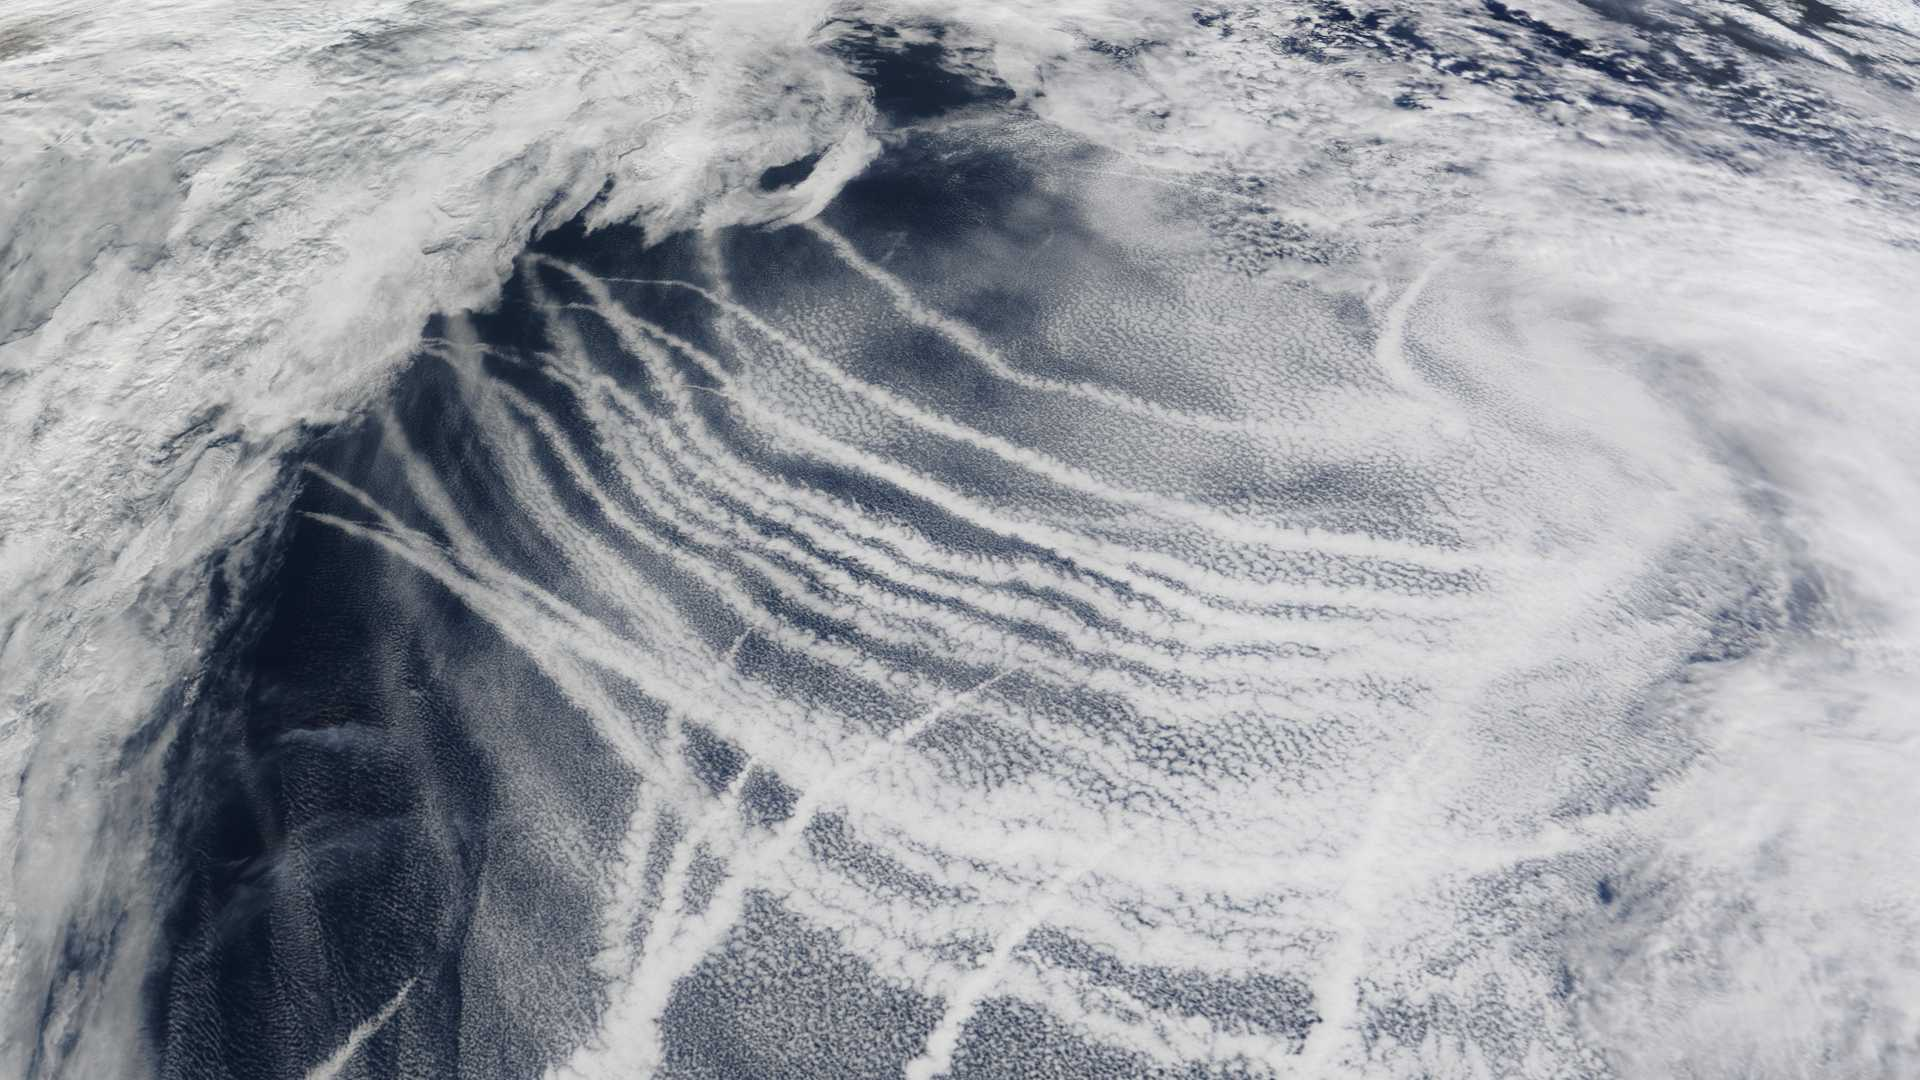
\includegraphics[width=0.65\textwidth]{figurer/ship_tracks.jpg}
\caption{\textit{Ship tracks observed by NASA's MODIS instrument on board the Aqua satellite. Figure retrieved from \url{https://svs.gsfc.nasa.gov/3667} October 9, 2019. More information about the instrument is found in Chapter \ref{ch:metode}.}}
\label{fig:shiptracks}
\end{figure}
\cite{glasius_composition_2018}

\section{Global modelling of ERFaci}
\subsection{Earth System Models}



